\documentclass[12pt, a4paper]{article}
\usepackage[margin=1in]{geometry}
\usepackage{graphicx}
\usepackage{booktabs}
\usepackage{listings}
\usepackage{xcolor}
\usepackage{hyperref}
\usepackage{amsmath}
\usepackage{algorithm}
\usepackage{algpseudocode}
\usepackage{float}

% Code listing style
\definecolor{codegreen}{rgb}{0,0.6,0}
\definecolor{codegray}{rgb}{0.5,0.5,0.5}
\definecolor{codepurple}{rgb}{0.58,0,0.82}
\definecolor{backcolour}{rgb}{0.95,0.95,0.92}

\lstdefinestyle{mystyle}{
    backgroundcolor=\color{backcolour},   
    commentstyle=\color{codegreen},
    keywordstyle=\color{magenta},
    numberstyle=\tiny\color{codegray},
    stringstyle=\color{codepurple},
    basicstyle=\ttfamily\footnotesize,
    breakatwhitespace=false,         
    breaklines=true,                 
    captionpos=b,                    
    keepspaces=true,                 
    numbers=left,                    
    numbersep=5pt,                  
    showspaces=false,                
    showstringspaces=false,
    showtabs=false,                  
    tabsize=2
}
\lstset{style=mystyle}

\title{\textbf{Auralis-DSA: Optimized Market Session Analyzer \& Trade Risk Engine}}
\author{
    Muntazir Mehdi (CMS: 503710) — Module 1 \\
    Muhammad Hannan Faisal (CMS: 507444) — Module 2 \\
    Muhammad Sammar Abbas (CMS: 509701) — Module 3
}
\date{
    CS-250 — Data Structures \& Algorithms \\
    Instructor: Dr. Ayesha Hakim \\
    \today
}

\begin{document}

\maketitle
\tableofcontents
\newpage

% ============================================================
\section{Introduction}
% ============================================================

\subsection{Problem Statement}
Financial markets generate large volumes of OHLC (Open, High, Low, Close) time-series data, requiring fast detection of session patterns (Asian, London, NY), candle range calculations, and dynamic risk handling across multiple trades. Manual analysis becomes slow and inaccurate as data grows.

\subsection{Project Objectives}
This project builds a Python-based DSA-driven market session analyzer that:
\begin{enumerate}
    \item Efficiently stores candle data using a \textbf{Dynamic Array} with $O(1)$ amortized insertion
    \item Classifies timestamps into trading sessions using an \textbf{AVL Tree} with $O(\log n)$ lookup
    \item Manages active trades using a \textbf{Linked List} and \textbf{Max-Heap} for priority-based risk management
\end{enumerate}

% ============================================================
\section{Data Structures \& Algorithms Used}
% ============================================================

\subsection{Summary Table}

\begin{table}[H]
\centering
\caption{Data Structures and Their Complexities}
\begin{tabular}{@{}llll@{}}
\toprule
\textbf{Module} & \textbf{Data Structure} & \textbf{Operation} & \textbf{Time Complexity} \\
\midrule
Module 1 & Dynamic Array & Insert (append) & Amortized $O(1)$ \\
Module 1 & CandleStore & Binary Search & $O(\log n)$ \\
Module 2 & AVL Tree & Insert & $O(\log n)$ \\
Module 2 & AVL Tree & Search & $O(\log n)$ \\
Module 3 & Linked List & Insert/Delete & $O(1)$ \\
Module 3 & Max-Heap & Insert/Extract & $O(\log n)$ \\
Module 3 & TradeManager & Risk Enforcement & $O(k \log n)$ \\
\bottomrule
\end{tabular}
\end{table}

% ============================================================
\section{Module 1: CandleStore (Dynamic Array + Binary Search)}
% ============================================================
\textit{Developed by: Muntazir Mehdi (CMS: 503710)}

\subsection{Overview}
The CandleStore module efficiently stores OHLC candle data using a custom Dynamic Array implementation with a doubling strategy for amortized $O(1)$ insertions.

\subsection{Dynamic Array Implementation}
The Dynamic Array uses a \textbf{doubling strategy} where capacity is doubled whenever the array becomes full:

\begin{algorithm}[H]
\caption{Dynamic Array Append}
\begin{algorithmic}[1]
\Procedure{Append}{element}
    \If{size == capacity}
        \State $\text{new\_capacity} \gets \text{capacity} \times 2$
        \State Resize(new\_capacity) \Comment{$O(n)$ but rare}
    \EndIf
    \State $\text{data[size]} \gets \text{element}$
    \State $\text{size} \gets \text{size} + 1$
\EndProcedure
\end{algorithmic}
\end{algorithm}

\subsection{Binary Search for Timestamp Lookup}
Binary search provides $O(\log n)$ lookup time for finding candles by timestamp:

\begin{algorithm}[H]
\caption{Binary Search Timestamp}
\begin{algorithmic}[1]
\Procedure{BinarySearch}{target\_timestamp}
    \State $left \gets 0$, $right \gets n - 1$, $result \gets -1$
    \While{$left \leq right$}
        \State $mid \gets (left + right) / 2$
        \If{$\text{candles}[mid].\text{timestamp} = target$}
            \State \Return $mid$
        \ElsIf{$\text{candles}[mid].\text{timestamp} < target$}
            \State $result \gets mid$
            \State $left \gets mid + 1$
        \Else
            \State $right \gets mid - 1$
        \EndIf
    \EndWhile
    \State \Return $result$
\EndProcedure
\end{algorithmic}
\end{algorithm}

\subsection{Results}
% Insert figure here
\begin{figure}[H]
    \centering
    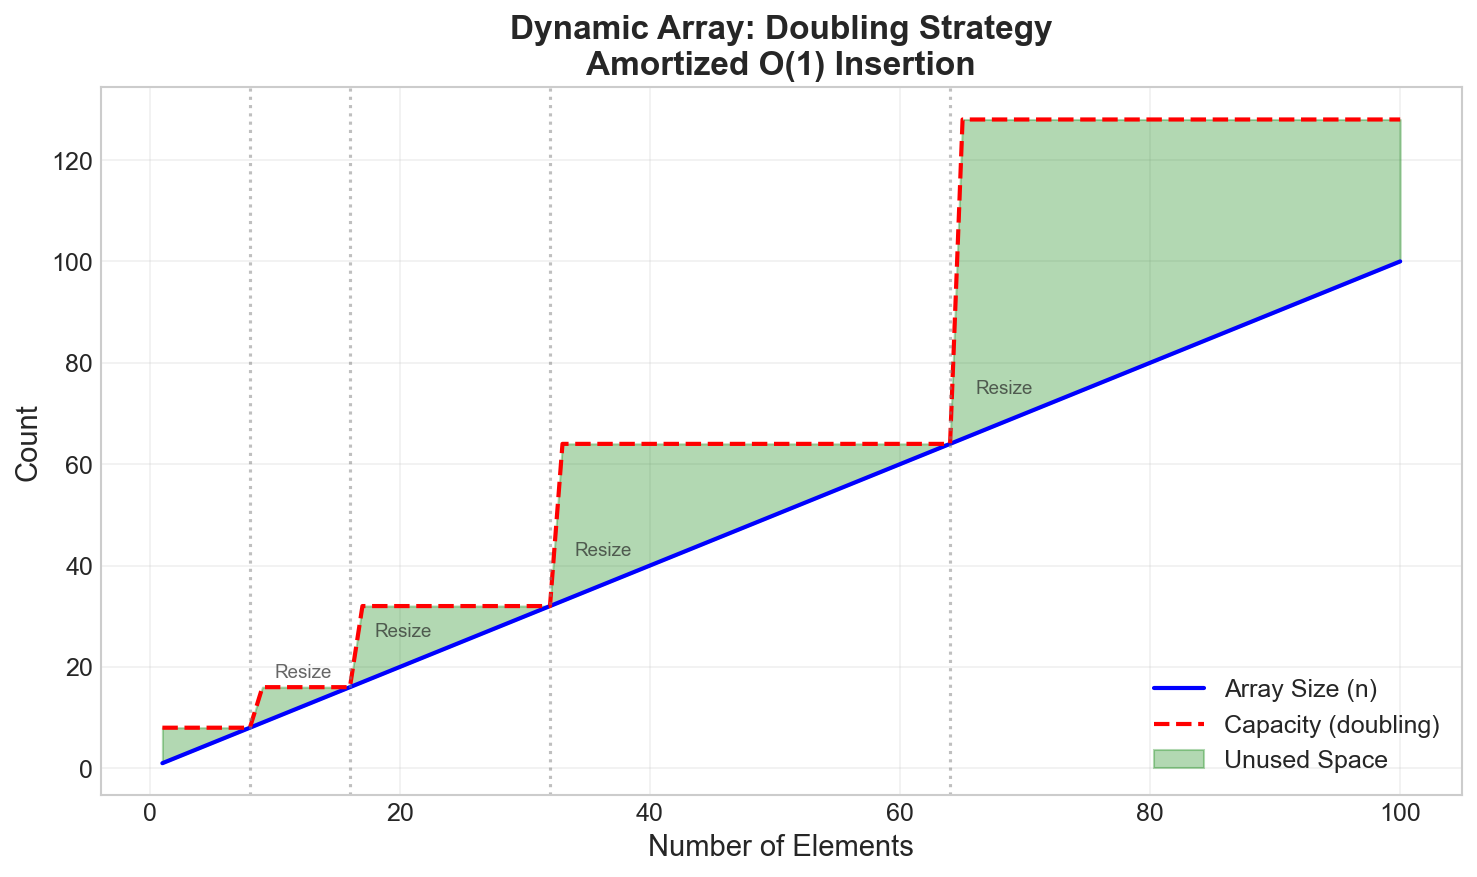
\includegraphics[width=0.8\textwidth]{plots/dsa_figures/dynamic_array_growth.png}
    \caption{Dynamic Array Growth with Doubling Strategy}
\end{figure}

\begin{figure}[H]
    \centering
    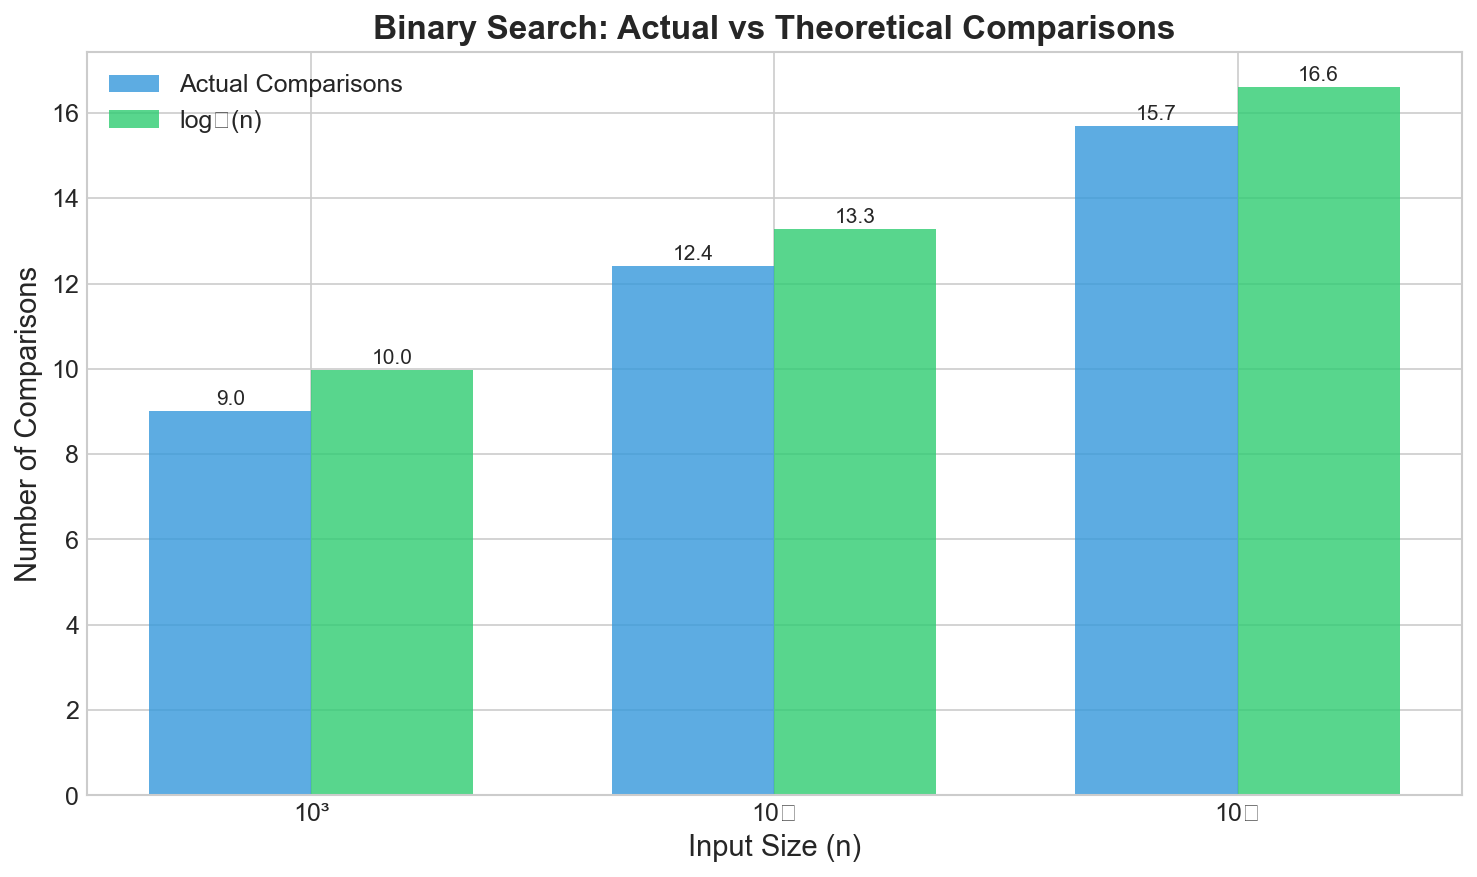
\includegraphics[width=0.8\textwidth]{plots/dsa_figures/binary_search_analysis.png}
    \caption{Binary Search: Actual vs Theoretical Comparisons}
\end{figure}

% ============================================================
\section{Module 2: SessionManager (AVL Tree)}
% ============================================================
\textit{Developed by: Muhammad Hannan Faisal (CMS: 507444)}

\subsection{Overview}
The SessionManager uses an AVL Tree (self-balancing BST) to classify timestamps into trading sessions with $O(\log n)$ lookup time.

\subsection{AVL Tree Rotations}
Four rotation cases are implemented to maintain balance:

\begin{enumerate}
    \item \textbf{Left-Left (LL):} Single right rotation
    \item \textbf{Right-Right (RR):} Single left rotation
    \item \textbf{Left-Right (LR):} Left rotation then right rotation
    \item \textbf{Right-Left (RL):} Right rotation then left rotation
\end{enumerate}

\begin{algorithm}[H]
\caption{AVL Right Rotation (LL Case)}
\begin{algorithmic}[1]
\Procedure{RotateRight}{y}
    \State $x \gets y.\text{left}$
    \State $B \gets x.\text{right}$
    \State $x.\text{right} \gets y$
    \State $y.\text{left} \gets B$
    \State UpdateHeight($y$)
    \State UpdateHeight($x$)
    \State \Return $x$
\EndProcedure
\end{algorithmic}
\end{algorithm}

\subsection{Tree Structure}
% Insert figure here
\begin{figure}[H]
    \centering
    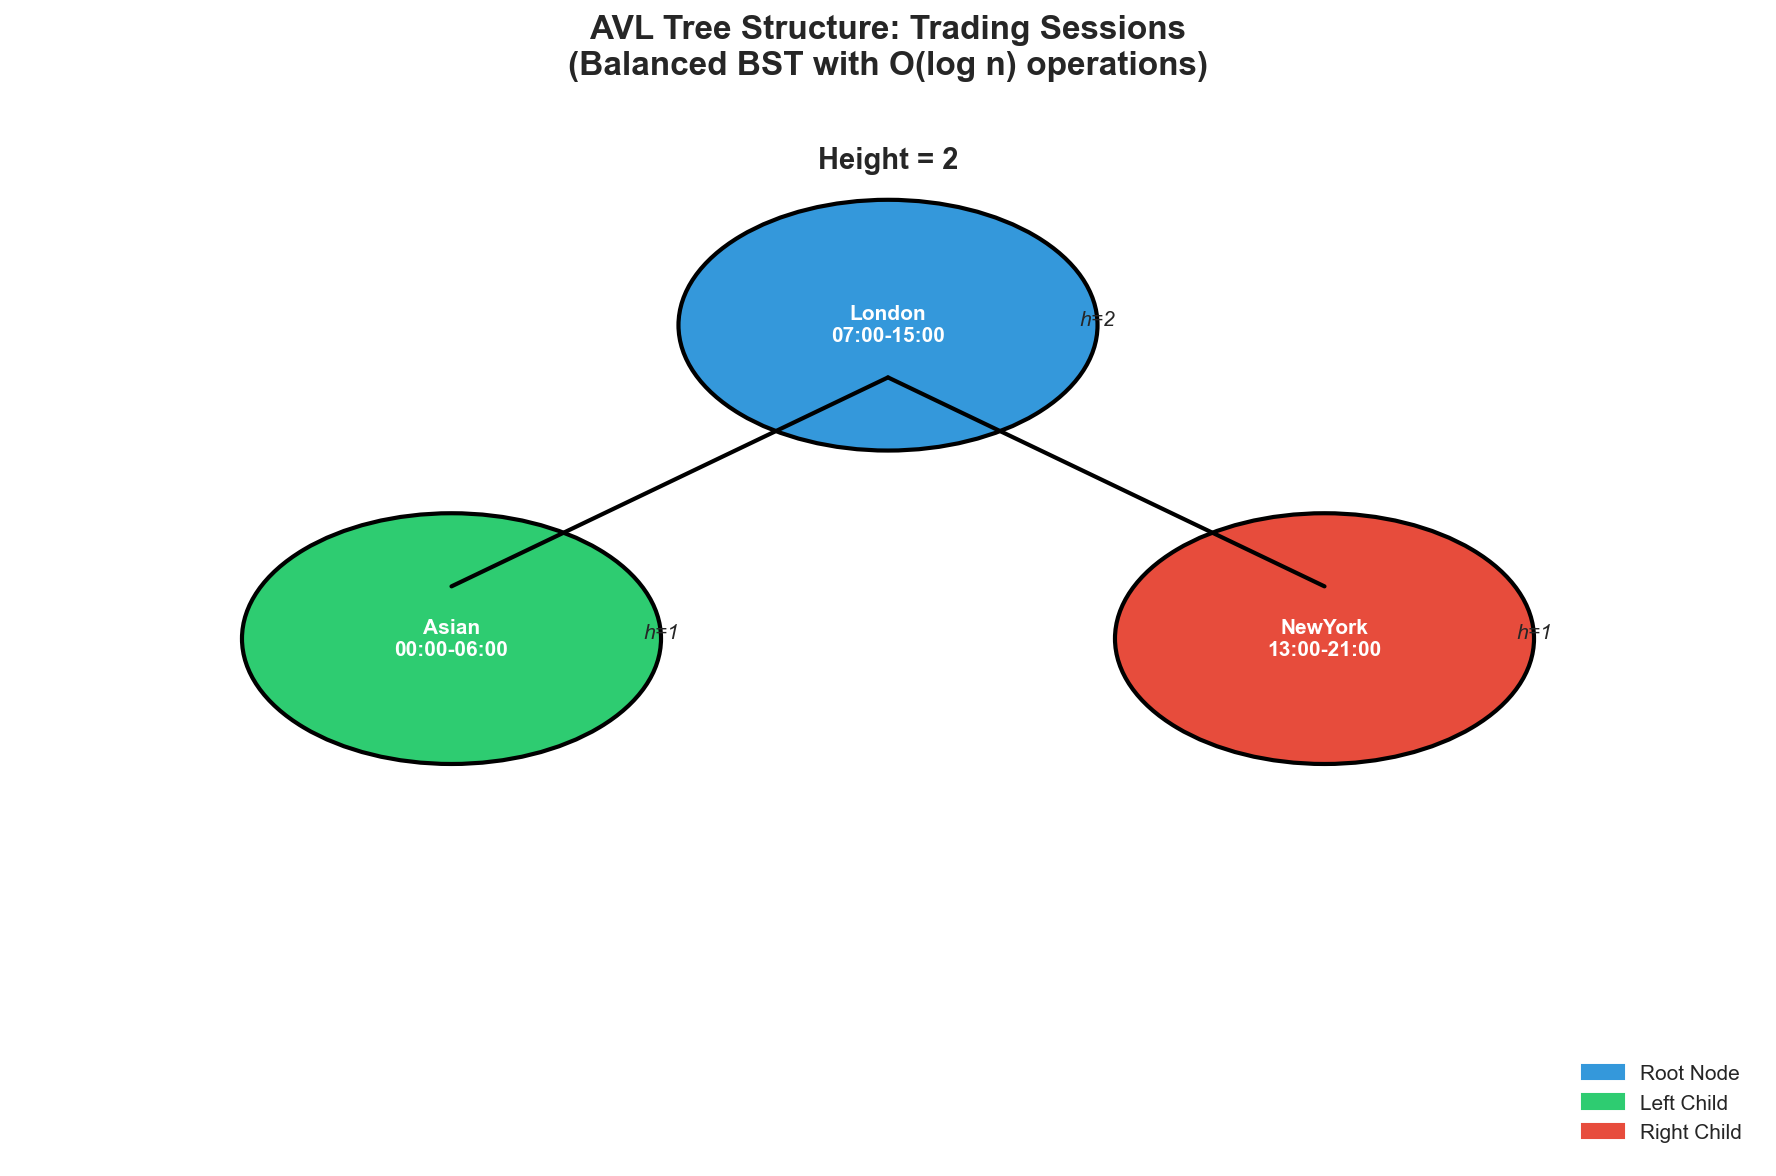
\includegraphics[width=0.7\textwidth]{plots/dsa_figures/avl_tree_structure.png}
    \caption{AVL Tree Structure for Trading Sessions}
\end{figure}

\subsection{Session Classification Output}
\begin{verbatim}
Hour (UTC)   Session         Comparisons
00:30        Asian           2
03:30        Asian           2
06:30        Off-Hours       2
09:30        London          1
12:30        London          1
15:30        NewYork         2
18:30        NewYork         2
\end{verbatim}

% ============================================================
\section{Module 3: TradeManager (Linked List + Max-Heap)}
% ============================================================
\textit{Developed by: Muhammad Sammar Abbas (CMS: 509701)}

\subsection{Overview}
The TradeManager combines a Doubly Linked List for $O(1)$ trade insertion/deletion with a Max-Heap for priority-based risk management.

\subsection{Doubly Linked List}
Provides $O(1)$ insertion and deletion with node reference:

\begin{algorithm}[H]
\caption{LinkedList Insert at Tail}
\begin{algorithmic}[1]
\Procedure{InsertTail}{trade}
    \State $\text{node} \gets \text{new Node(trade)}$
    \If{tail = null}
        \State $\text{head} \gets \text{tail} \gets \text{node}$
    \Else
        \State $\text{node.prev} \gets \text{tail}$
        \State $\text{tail.next} \gets \text{node}$
        \State $\text{tail} \gets \text{node}$
    \EndIf
    \State $\text{size} \gets \text{size} + 1$
\EndProcedure
\end{algorithmic}
\end{algorithm}

\subsection{Max-Heap for Risk Prioritization}
The Max-Heap keeps the highest-risk trade at the root for $O(1)$ access:

\begin{algorithm}[H]
\caption{Greedy Risk Enforcement}
\begin{algorithmic}[1]
\Procedure{EnforceRiskBudget}{}
    \While{total\_risk $>$ max\_budget \textbf{and} heap not empty}
        \State $\text{trade} \gets \text{heap.extract\_max()}$ \Comment{$O(\log n)$}
        \State Remove trade from linked list \Comment{$O(1)$}
        \State $\text{total\_risk} \gets \text{total\_risk} - \text{trade.risk}$
    \EndWhile
\EndProcedure
\end{algorithmic}
\end{algorithm}

\subsection{Results}
\begin{figure}[H]
    \centering
    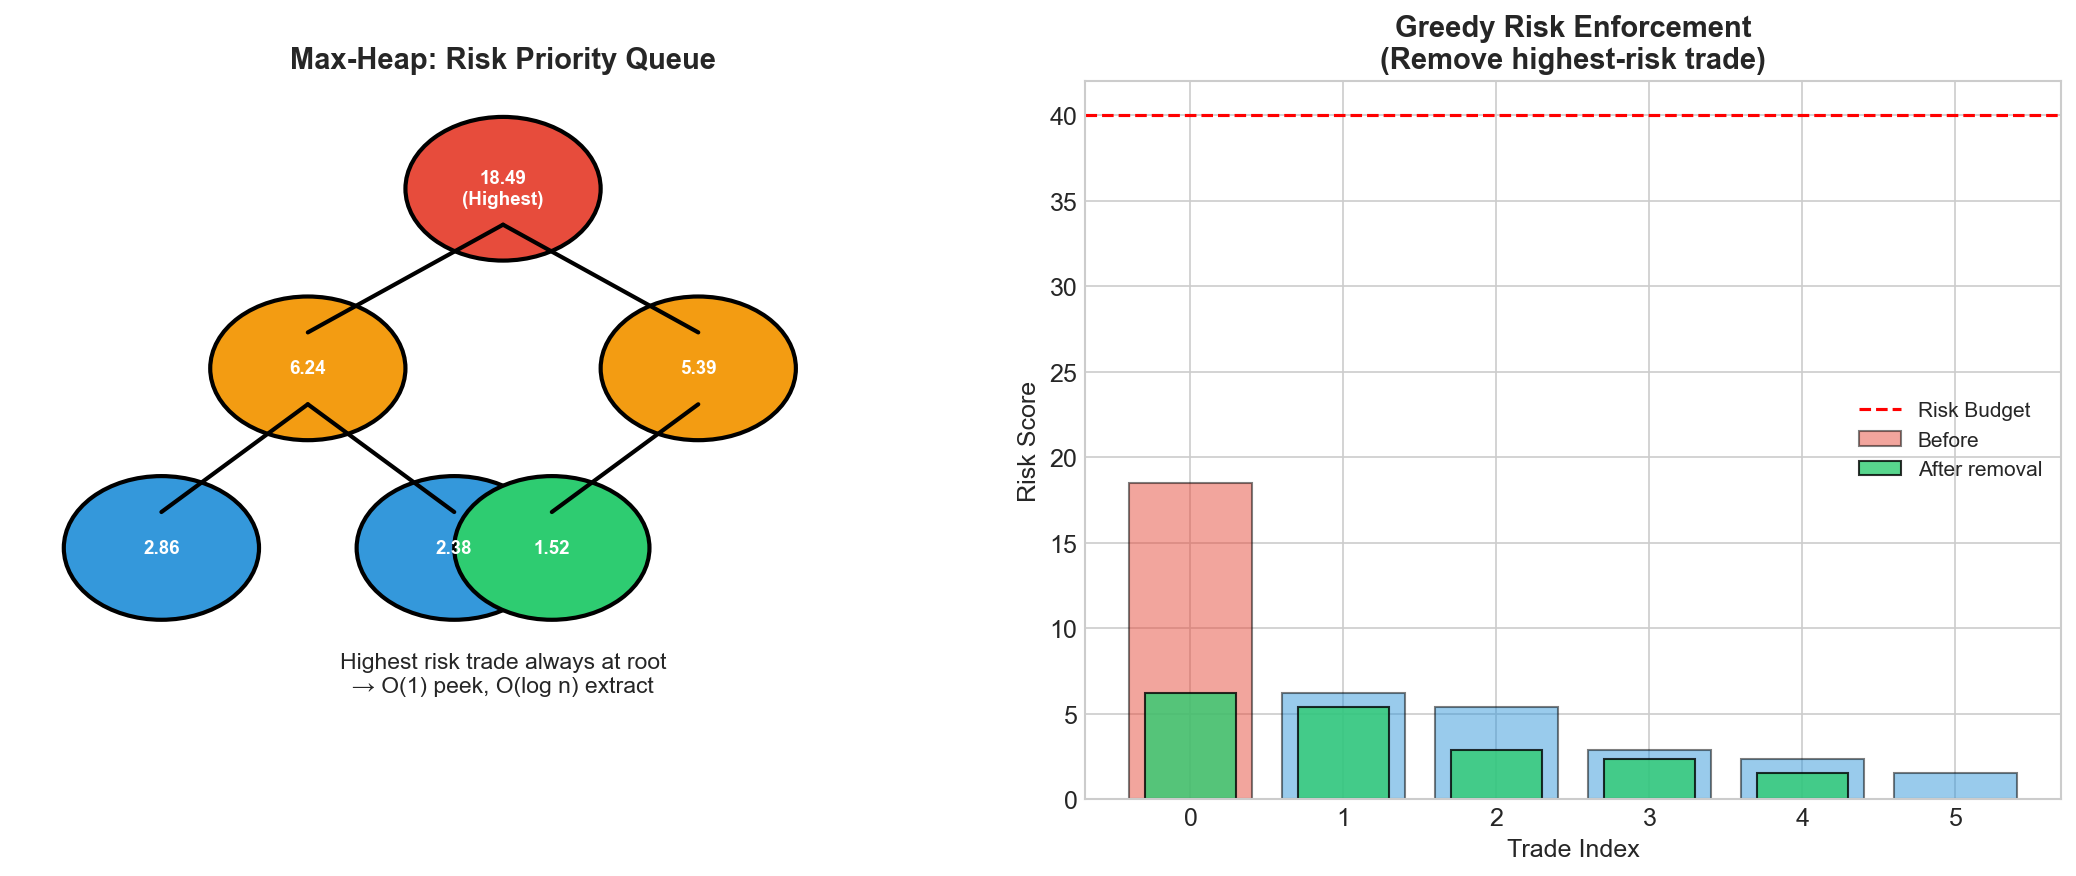
\includegraphics[width=\textwidth]{plots/dsa_figures/risk_heap_visualization.png}
    \caption{Max-Heap Risk Prioritization and Greedy Enforcement}
\end{figure}

% ============================================================
\section{Performance Benchmarks}
% ============================================================

\subsection{Test Configuration}
All benchmarks were run on input sizes: $n = 10^3, 10^4, 10^5$

\subsection{Benchmark Results}

\begin{figure}[H]
    \centering
    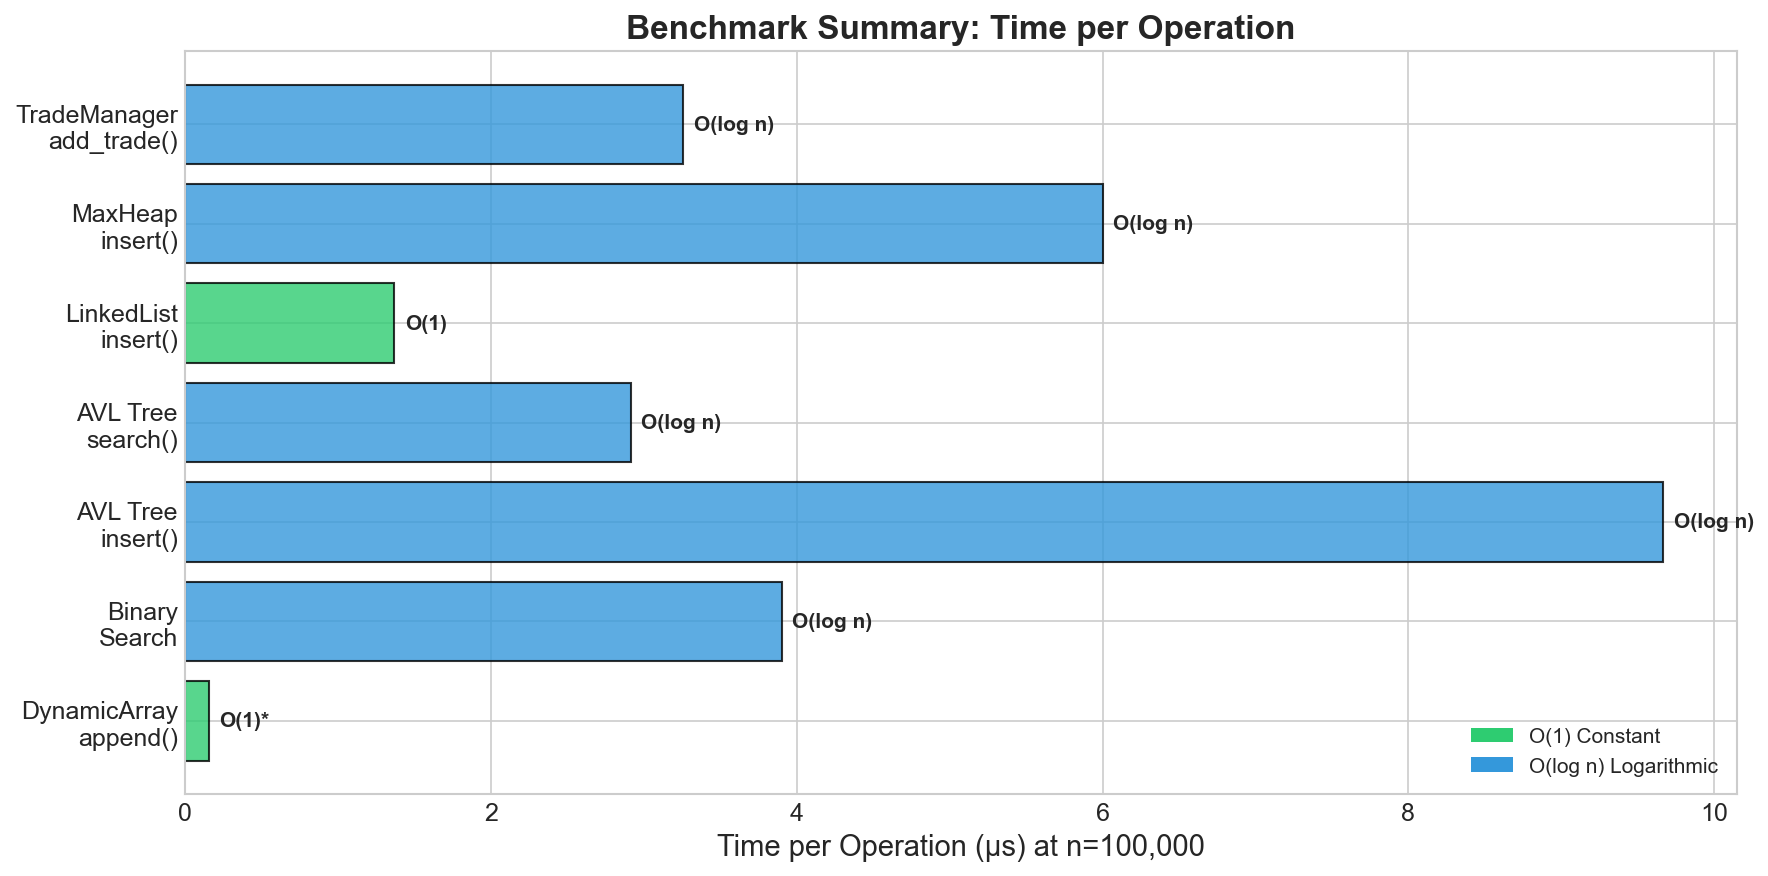
\includegraphics[width=0.9\textwidth]{plots/dsa_figures/benchmark_summary.png}
    \caption{Benchmark Summary: Time per Operation at $n=100,000$}
\end{figure}

\begin{figure}[H]
    \centering
    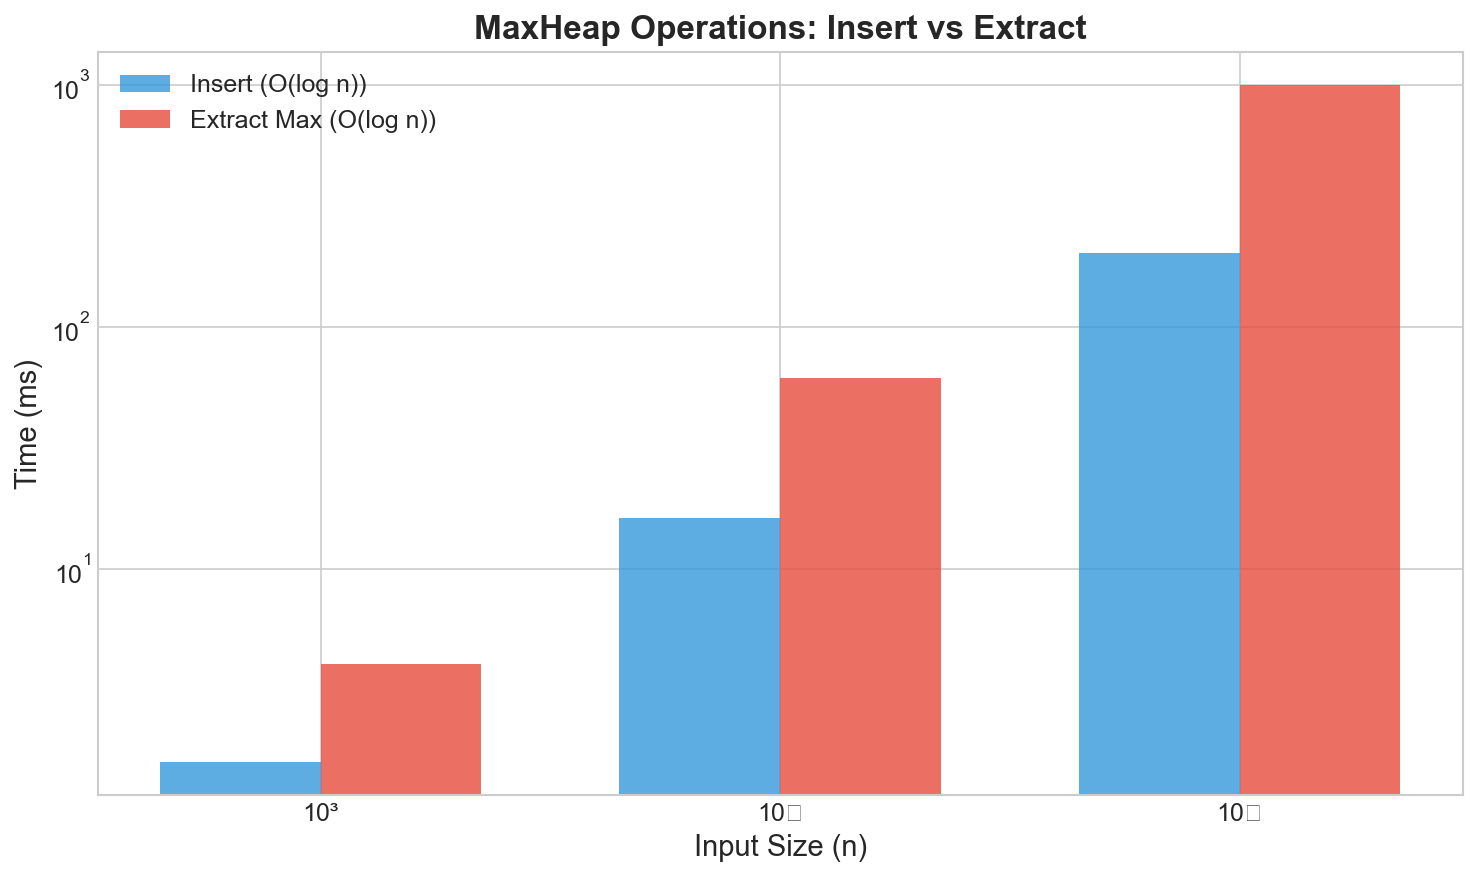
\includegraphics[width=0.9\textwidth]{plots/dsa_figures/heap_operations.png}
    \caption{MaxHeap Insert vs Extract Performance}
\end{figure}

\subsection{Complexity Verification}

\begin{table}[H]
\centering
\caption{Big-O Complexity Verification}
\begin{tabular}{@{}llcc@{}}
\toprule
\textbf{Data Structure} & \textbf{Operation} & \textbf{Expected} & \textbf{Verified} \\
\midrule
DynamicArray & append() & $O(1)^*$ & \checkmark \\
CandleStore & binary\_search() & $O(\log n)$ & \checkmark \\
AVL Tree & insert() & $O(\log n)$ & \checkmark \\
AVL Tree & search() & $O(\log n)$ & \checkmark \\
LinkedList & insert\_tail() & $O(1)$ & \checkmark \\
MaxHeap & insert() & $O(\log n)$ & \checkmark \\
MaxHeap & extract\_max() & $O(\log n)$ & \checkmark \\
MaxHeap & peek\_max() & $O(1)$ & \checkmark \\
\bottomrule
\end{tabular}
\end{table}

\begin{figure}[H]
    \centering
    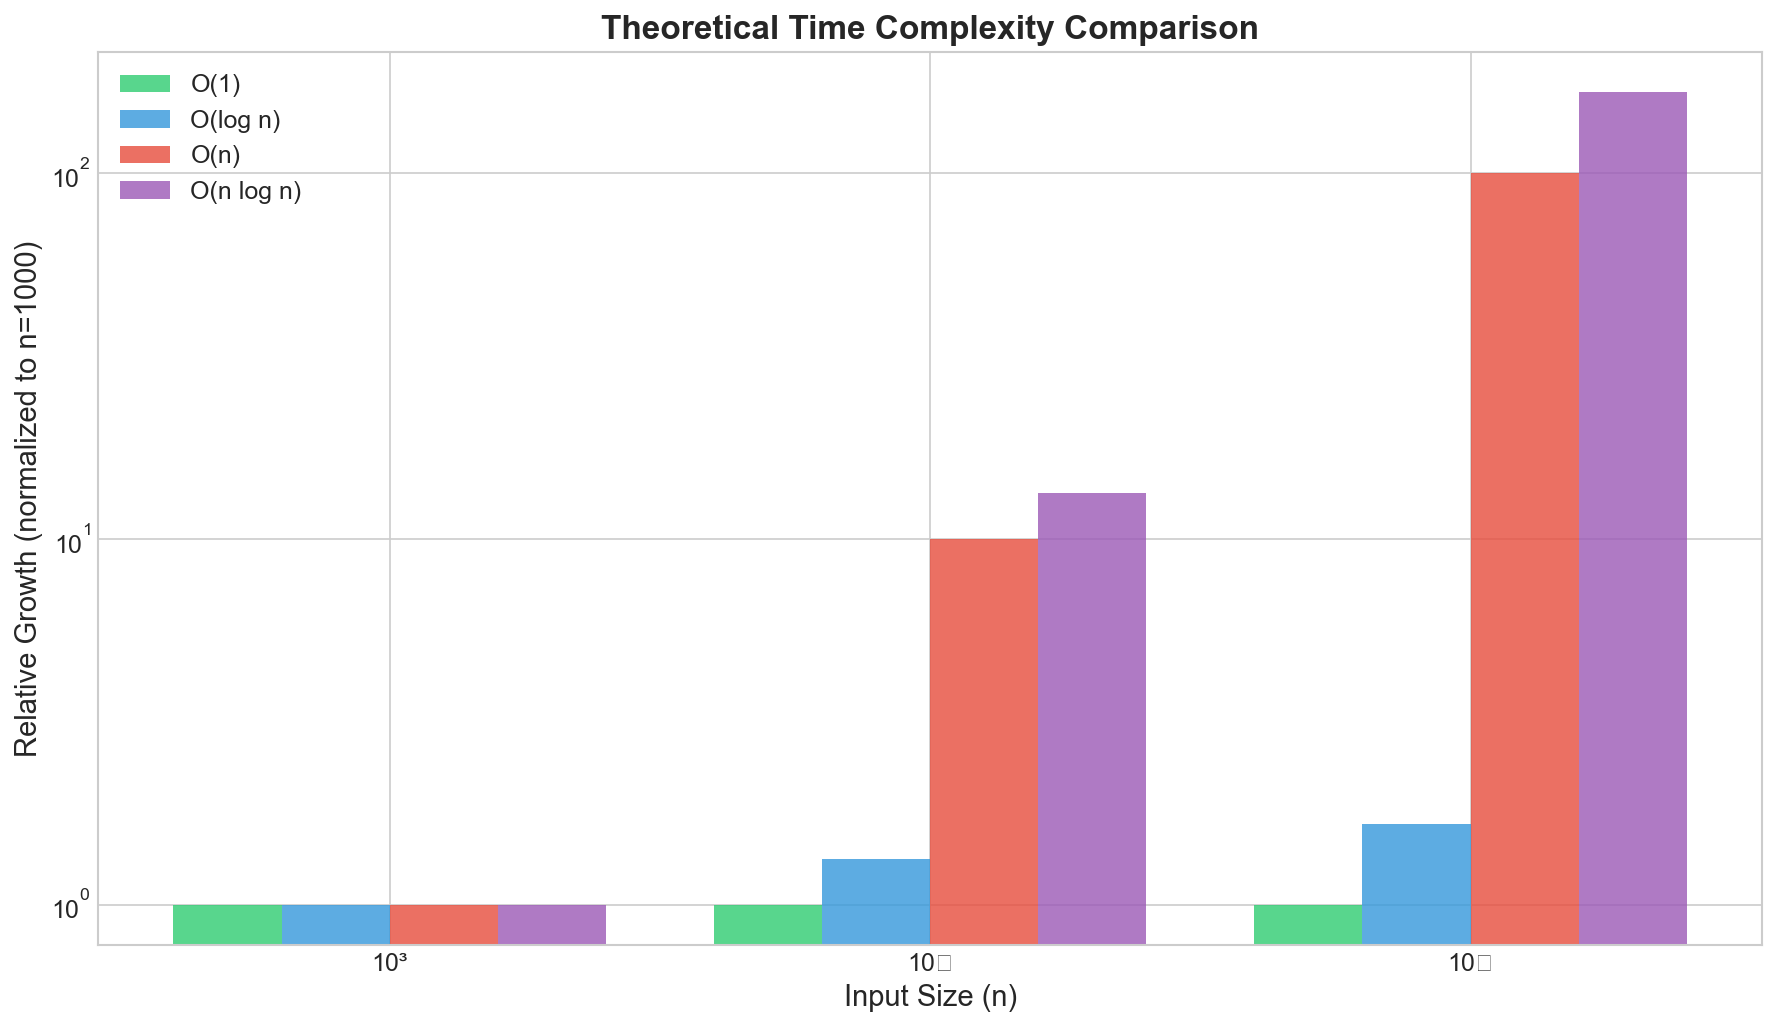
\includegraphics[width=0.9\textwidth]{plots/dsa_figures/complexity_comparison.png}
    \caption{Theoretical Time Complexity Comparison}
\end{figure}

% ============================================================
\section{Integrated Workflow}
% ============================================================

The three modules work together in a complete trading workflow:

\begin{enumerate}
    \item \textbf{Data Loading:} XAUUSD M5 candles loaded into CandleStore (828,000 candles)
    \item \textbf{Session Detection:} AVL Tree classifies each timestamp (Asian/London/NY)
    \item \textbf{Trade Execution:} Trades added to LinkedList + MaxHeap
    \item \textbf{Risk Management:} Greedy algorithm enforces risk limits
\end{enumerate}

% ============================================================
\section{Conclusion}
% ============================================================

This project successfully demonstrates the application of fundamental data structures and algorithms to a real-world financial trading system:

\begin{itemize}
    \item \textbf{Dynamic Array} with doubling strategy provides amortized $O(1)$ insertion
    \item \textbf{Binary Search} enables $O(\log n)$ timestamp lookups in sorted candle data
    \item \textbf{AVL Tree} maintains balanced structure for $O(\log n)$ session classification
    \item \textbf{Doubly Linked List} provides $O(1)$ trade management operations
    \item \textbf{Max-Heap} enables efficient priority-based risk management
    \item \textbf{Greedy Algorithm} optimally enforces risk budget constraints
\end{itemize}

All data structures were \textbf{manually implemented} without using Python's built-in equivalents (heapq, collections.deque, etc.).

% ============================================================
\section{References}
% ============================================================

\begin{enumerate}
    \item Cormen, T.H., et al. \textit{Introduction to Algorithms}, 3rd Edition. MIT Press.
    \item Sedgewick, R., \& Wayne, K. \textit{Algorithms}, 4th Edition. Addison-Wesley.
\end{enumerate}

\end{document}
